\section{Proposed Approach}

This section gives the details about our proposed method which aims at detecting counterfeit fingerprints from applications' outbound HTTP traffics. The proposed counterfeit fingerprint detection process consists of training and testing phases. In training phase, we assume enterprise hosts aren't compromised. This method mainly arises from the first one that is a data-driven and unsupervised flow responsible for a browser's fingerprint \cite{bortolameotti2017decanter} and referrer correlation construction. This step takes the fields of a PCAP file as input and classifies browser traffics, and then construct fingerprints and referrer correlation graphs. In the testing phase, given a browser outbound HTTP traffic reconstructed by fingerprint and referrer correlation graph, and the second step filters benign browser traffics through fingerprint matching. Continuously, compare its and trained referrer correlation graph using Graph Edit Distance (GED) for counterfeit fingerprint detection. The proposed method is depicted in figure \ref{fig:sa} and following paragraphs describe the details of each component.

\begin{figure*}[!t]
\centering
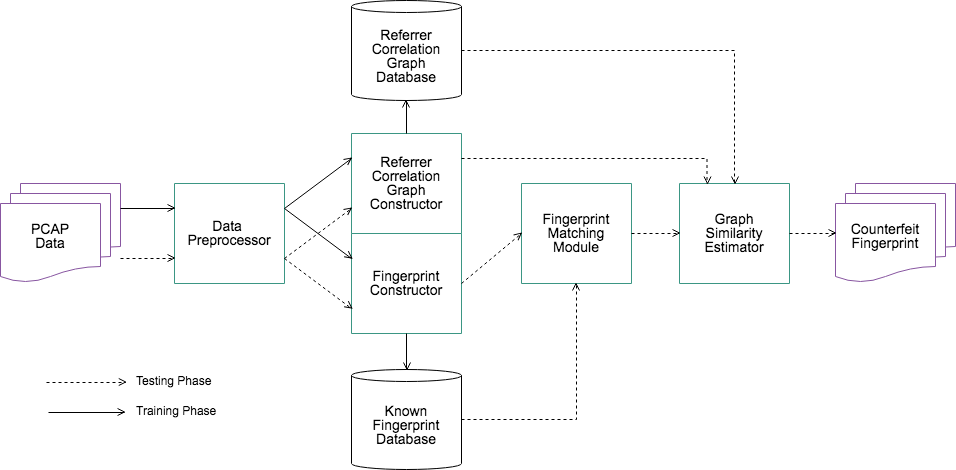
\includegraphics[width=400pt]{image/sa.png}
\caption{An overview of our counterfeit fingerprint detection system. Five subsystems are depicted: (1) PCAP data preprocessor subsystem, (2) benign fingerprint constructor subsystem, (3) benign traffic extractor subsystem, (4) referrer correlation graph constructor subsystem, and (5) graph similarity estimator subsystem. The system only takes the PCAP files of outbound HTTP traffics as input. In training phase, subsystem (1) and (2) passively extract the benign fingerprint from an application's outbound HTTP traffic, and subsystem (3) could use fingerprints to classify benign traffic in the testing phase. We note that referrer correlation extraction in the subsystem (4) is a key step, in the sense that if it can extract discriminative features for counterfeit fingerprint detection, the detection in the subsystem (5) is relatively straightforward.}
\label{fig:sa}
\end{figure*}

\subsection{PCAP Data Preprocessor}

\subsection{Benign Fingerprint Constructor}

\subsection{Benign Traffic Extractor}

\subsection{Referrer Correlation Graph Constructor}

\subsection{Graph Similarity Estimator}